\begin{tcolorbox}[
  enhanced,
  breakable,
  colback=gray!6,
  colframe=chaptercolor,
  boxrule=0.8pt,
  arc=3pt,
  title={Guide to Appendix~\ref{chap:appendix-privpgd}},
  colbacktitle=chaptercolor!12,
  coltitle=black
]
This appendix is organized in six parts:
\begin{itemize}
  \item descriptions and preprocessing steps for the nine tabular benchmarks;
  \item implementation and hyperparameter details for PrivPGD and the baselines;
  \item technical notes on projection, quantization, finalization, and the proof of \Cref{lem:privpgd-privacy};
  \item setup and regularization details for the constrained synthesis experiment;
  \item benchmark and distance comparison figures at \(\epsilon = 1.0\) and \(\epsilon = 0.2\); and
  \item full numerical benchmark tables for \(\epsilon = 2.5\), \(1.0\), and \(0.2\).
\end{itemize}
\end{tcolorbox}

\section{Datasets and Preprocessing}
\label{app:privpgd-datasets}

The empirical study uses nine real-world tabular datasets drawn from the American Community Survey (ACS) and from the tabular benchmark of \citet{grinsztajn2022tree}. Unless noted otherwise, each dataset is split into \(80\%\) sensitive training data and \(20\%\) held-out test data. Real-valued variables, as well as integer-valued variables with range larger than \(32\), are discretized into \(32\) equally sized bins before private release.

\subsection{Classification benchmarks}
\begin{itemize}
  \item \textbf{ACS Income (Inc.)}~\citep{ding2021retiring}. This task predicts whether an individual earns more than \$50,000 per year. The dataset is derived from the ACS PUMS sample after filtering to individuals older than 16 who reported at least one hour of work per week in the preceding year and reported annual income above \$100. The benchmark uses California data from survey year 2018 with a five-year horizon, yielding \(d=11\) features and \(n=760{,}157\) records.
  \item \textbf{ACS Employment (Emp.)}~\citep{ding2021retiring}. This task predicts employment status. The sample is restricted to individuals aged 16 to 90 from the California 2018 five-year ACS release. The resulting dataset has \(d=17\) features and \(n=1{,}503{,}938\) records.
  \item \textbf{ACS Mobility (Mob.)}~\citep{ding2021retiring}. This task predicts whether an individual kept the same residential address as in the previous year. To avoid a nearly trivial class imbalance, the benchmark restricts attention to individuals aged 18 to 35. The California 2018 five-year release yields \(d=22\) features and \(n=318{,}332\) records.
  \item \textbf{ACS Traveltime (Tra.)}~\citep{ding2021retiring}. This task predicts whether an individual has a work commute longer than 20 minutes. The sample is restricted to employed individuals older than 16, and the 20-minute threshold corresponds to the national median commute time in the 2018 ACS PUMS release. The California 2018 five-year data yield \(d=17\) features and \(n=667{,}132\) records.
  \item \textbf{ACS Public Coverage (Pub.)}~\citep{ding2021retiring}. This task predicts whether an individual is enrolled in public health insurance. The benchmark focuses on individuals younger than 65 with income below \$30,000 so that the task targets low-income individuals not eligible for Medicare. The California 2018 five-year release yields \(d=20\) features and \(n=583{,}545\) records.
  \item \textbf{Diabetes 130-US (Diab.)}~\citep{strack2014impact}. This task uses ten years of inpatient records from 130 US hospitals and integrated delivery systems. The curation keeps admissions associated with a diabetes diagnosis, hospital stays between 1 and 14 days, laboratory tests, and medication administration. The resulting benchmark has \(d=7\) features and \(n=56{,}872\) records.
\end{itemize}

\subsection{Regression benchmarks}
\begin{itemize}
  \item \textbf{Medical Charges (Med.)}~\citep{grinsztajn2022tree}. This dataset is derived from the Inpatient Utilization and Payment Public Use File and records inpatient discharges under Medicare fee-for-service. It covers more than 3,000 hospitals under the Medicare Inpatient Prospective Payment System from fiscal years 2011 to 2016. The benchmark uses \(d=3\) features and \(n=130{,}452\) records.
  \item \textbf{Black Friday (Fri.)}~\citep{grinsztajn2022tree}. This task uses purchase records from \(n=133{,}456\) buyers and \(d=9\) features, including gender, age, occupation, and marital status.
  \item \textbf{NYC Taxi Green December 2016 (Taxi)}~\citep{grinsztajn2022tree}. This dataset is derived from New York City Taxi and Limousine Commission records for green-line trips in December 2016. The target is the tip amount, and only credit-card trips are retained. The processed dataset has \(d=9\) features and \(n=465{,}468\) records.
\end{itemize}

\section{Implementation Details}
\label{app:privpgd-implementation}

This section records the concrete experimental settings that were omitted from the main chapter to keep the narrative focused on the main results.

\subsection{Shared experimental protocol}
All benchmark results are averaged over five runs. The primary privacy setting is \(\epsilon = 2.5\) and \(\delta = 10^{-5}\), while the lower-budget replications reported below use the same \(\delta\) and smaller values of \(\epsilon\). Downstream task performance is measured by training a gradient-boosting model on the synthetic data and evaluating it on the held-out test split (0-1 error for classification and mean squared error for regression). We use the \texttt{scikit-learn} implementation \citep{sklearn_api} with standard hyperparameters, and all evaluation is carried out on the discretized representation of the data.

\subsection{PrivPGD configuration}
PrivPGD is implemented in \texttt{PyTorch} (code available at \url{https://github.com/jaabmar/private-pgd}) and run on a GPU with fixed hyperparameters across all datasets. For all datasets, the released statistics consist of all two-way marginals, privatized with the Gaussian mechanism. The synthetic release is represented by \(100{,}000\) particles.

For the projection step, the sliced \(1\)-Wasserstein distance is approximated with \(200\) Monte Carlo projection directions. The projected probability measure is computed with \texttt{Adam} for \(1750\) iterations, using an initial learning rate of \(0.1\) and a linear scheduler with step size \(100\) and multiplicative factor \(0.8\). The initialization clips negative weights of the embedded signed marginal to zero and renormalizes the remaining positive mass.

For the optimization step, the squared sliced \(2\)-Wasserstein loss is approximated with \(N_{\mathrm{MC}} = 10\) projection directions. The particle cloud is optimized for \(1000\) epochs, with each epoch visiting every selected marginal once. The subsets in \(\mathcal{S}\) are processed in mini-batches of size \(5\). The optimizer uses an initial learning rate of \(0.1\), a linear scheduler with step size \(50\) and multiplicative factor \(0.75\), and \texttt{Sparse Adam}. At each update, \(80\%\) of the gradient entries are randomly set to zero.

\subsection{Baseline configurations}
MST and AIM are run with the authors' official implementation, available at \url{https://github.com/ryan112358/private-pgm}, with all two-way marginals as the workload for AIM. The mirror-descent optimizer is run for \(3000\) iterations with initial learning rate \(1.0\) and fixed hyperparameters across all datasets, and the sensitivity constants in the Gaussian and exponential mechanisms are adjusted so that the implementation matches the privacy model in \Cref{def:privpgd-dp}.

For Private GSD, GEM, and RAP, all two-way marginals are used as the query set, and hyperparameters are fine-tuned for each dataset over grids that include the configurations considered by \citet{pmlr-v202-liu23ag}. Private GSD is run in its one-shot variant with elite size \(2\) and early stopping. The tuned hyperparameters are the number of generations \(G \in \{200\mathrm{k}, 500\mathrm{k}\}\), mutation and crossover population sizes \(P_{\mathrm{mut}} = P_{\mathrm{cross}} \in \{50, 100, 150, 200, 500\}\), and the synthetic dataset size \(m \in \{2\mathrm{k}, 100\mathrm{k}\}\). For GEM and RAP, the official implementations are used with their default settings, while tuning the iteration counts \(T \in \{3, 10, 30, 50, 100, 150, 200\}\). For GEM, the model architecture is tuned over \([512, 512, 1024]\) and \([128, 256]\). For RAP, the learning rate is tuned over \(\{0.0001, 0.001, 0.03\}\) and the synthetic dataset size over \(\{2\mathrm{k}, 500\mathrm{k}\}\). GEM and RAP could not be run on the ACS Employment dataset under the available \(20\) GB memory budget.

\clearpage
\section{Technical Notes}
\label{app:privpgd-technical}

This section records technical details that complement the main chapter.

\subsection{Projection and quantization}
In implementation, each embedded signed measure is initialized by clipping negative mass and renormalizing. This only provides a feasible starting point for the optimization that minimizes the sliced \(1\)-Wasserstein distance to the embedded signed measure. After projection, the resulting probability measure is quantized to the same number of support points as the synthetic particle cloud so that the optimization stage compares empirical measures of the same size.

\subsection{Finalization}
After optimization in the embedded space, each particle is mapped to the nearest point of the embedded discrete grid before decoding. This ensures that the released synthetic dataset is again a genuine tabular dataset.

\subsection{Privacy guarantee}
\label{app:privpgd-privacy}
The privacy guarantee of PrivPGD follows from basic composition and the post-processing property of differential privacy \citep{dwork2014algorithmic}.

\begin{proof}[Proof of \Cref{lem:privpgd-privacy}]
Let the privatized marginals be released by an \((\epsilon_1,\delta_1)\)-differentially private mechanism, and let an optional auxiliary regularization statistic be released by an \((\epsilon_2,\delta_2)\)-differentially private mechanism. By basic composition \citep{dwork2014algorithmic}, their joint release is \((\epsilon_1+\epsilon_2,\delta_1+\delta_2)\)-differentially private. PrivPGD then applies only post-processing to these released objects: embedding, projection, quantization, gradient-based optimization, and final discretization. By the post-processing property of differential privacy \citep{dwork2014algorithmic}, the final synthetic dataset inherits the same \((\epsilon_1+\epsilon_2,\delta_1+\delta_2)\)-differential privacy guarantee. In the unregularized setting, the second mechanism is absent.
\end{proof}

\clearpage
\section{Constrained Synthesis Details}
\label{app:privpgd-constraints}

\subsection{Target statistic and smooth surrogate}

The constrained synthesis experiment from the main chapter augments the standard PrivPGD objective with a differentiable penalty designed to make a chosen population-level threshold statistic differ from its value on the sensitive data. For any integer \(r \geq 1\) and point cloud \(Z = (z_1,\dots,z_r) \in \Omega^r\), the target statistic in the embedded space is
\[
  q_{\theta,b}(Z)
  =
  \frac{1}{r}\sum_{j=1}^r \mathbf{1}\!\left\{\langle z_j, \theta \rangle + b > 0\right\}.
\]
Because this quantity is not differentiable with respect to the particle positions, the implementation replaces it by a smooth surrogate based on the same affine score,
\[
  \tilde q_{\theta,b}(Z)
  =
  \frac{1}{r}\sum_{j=1}^r
  \left(1 + \exp\!\left(-\kappa(\langle z_j, \theta \rangle + b)\right)\right)^{-1},
\]
with smoothing parameter \(\kappa = 5.0\).

\subsection{Privacy split and regularized objective}

The privacy budget is split between the auxiliary threshold statistic and the marginal release. A budget of \(\epsilon = 0.5\) and \(\delta = 2 \times 10^{-6}\) is used to obtain a differentially private estimate \(\widehat{\tilde q}_{\theta,b}(D)\) of \(\tilde q_{\theta,b}(\Emb(D))\) via the Gaussian mechanism. The remaining budget, \(\epsilon = 2.0\) and \(\delta = 8 \times 10^{-6}\), is used to privatize all two-way marginals. By simple composition, the overall constrained release therefore remains \((2.5,10^{-5})\)-differentially private.

The regularization term optimized in this experiment is
\[
  \hat{\mathcal{R}}_{\mathrm{constr}}(Z)
  =
  \frac{0.01}{0.0001 + \left(\tilde q_{\theta,b}(Z) - \widehat{\tilde q}_{\theta,b}(D)\right)^2},
\]
and the reported sweeps vary the regularization strength \(\lambda\) from \(10^{-2}\) to \(10^{2}\) (that is, \(\log_{10}\lambda \in \{-2, -1, 0, 1, 2\}\)). Since this term is added to a loss that is minimized, increasing \(\lambda\) encourages a larger discrepancy between the synthetic statistic and the differentially private estimate of the sensitive statistic. The resulting tradeoff curves for the ACS Income and ACS Employment datasets are shown in Figure~\ref{fig:constraints-main} in Chapter~\ref{chap:privpgd}.

\clearpage
\section{Lower-Budget Experiments}
\label{app:privpgd-low-eps}

The main chapter focuses on \(\epsilon = 2.5\), which is the regime in which PrivPGD is most competitive. At smaller privacy budgets, the relative advantage narrows, and the lower-\(\epsilon\) experiments help clarify the method's limitations as well as its strengths.

\subsection{\texorpdfstring{$\epsilon = 1.0$}{epsilon = 1.0}}

At \(\epsilon = 1.0\) (Figures~\ref{fig:app-privpgd-comp-1} and \ref{fig:app-privpgd-dist-1}), PrivPGD remains broadly competitive, but PGM-based methods, especially AIM, become stronger on a larger fraction of datasets. Private GSD also closes the gap on several tasks. This pattern is consistent with the stronger inductive bias of maximum-entropy-style PGM methods when the privatized marginals become noisier. Even so, PrivPGD remains particularly competitive on larger datasets and on settings in which geometry-aware fidelity is more informative than purely count-based matching.

\begin{figure}[!tbp]
  \centering
  
\includegraphics[width=0.9\textwidth]{papers/PrivPGD/figures/exp12legend_plot.pdf}\\[1ex]
  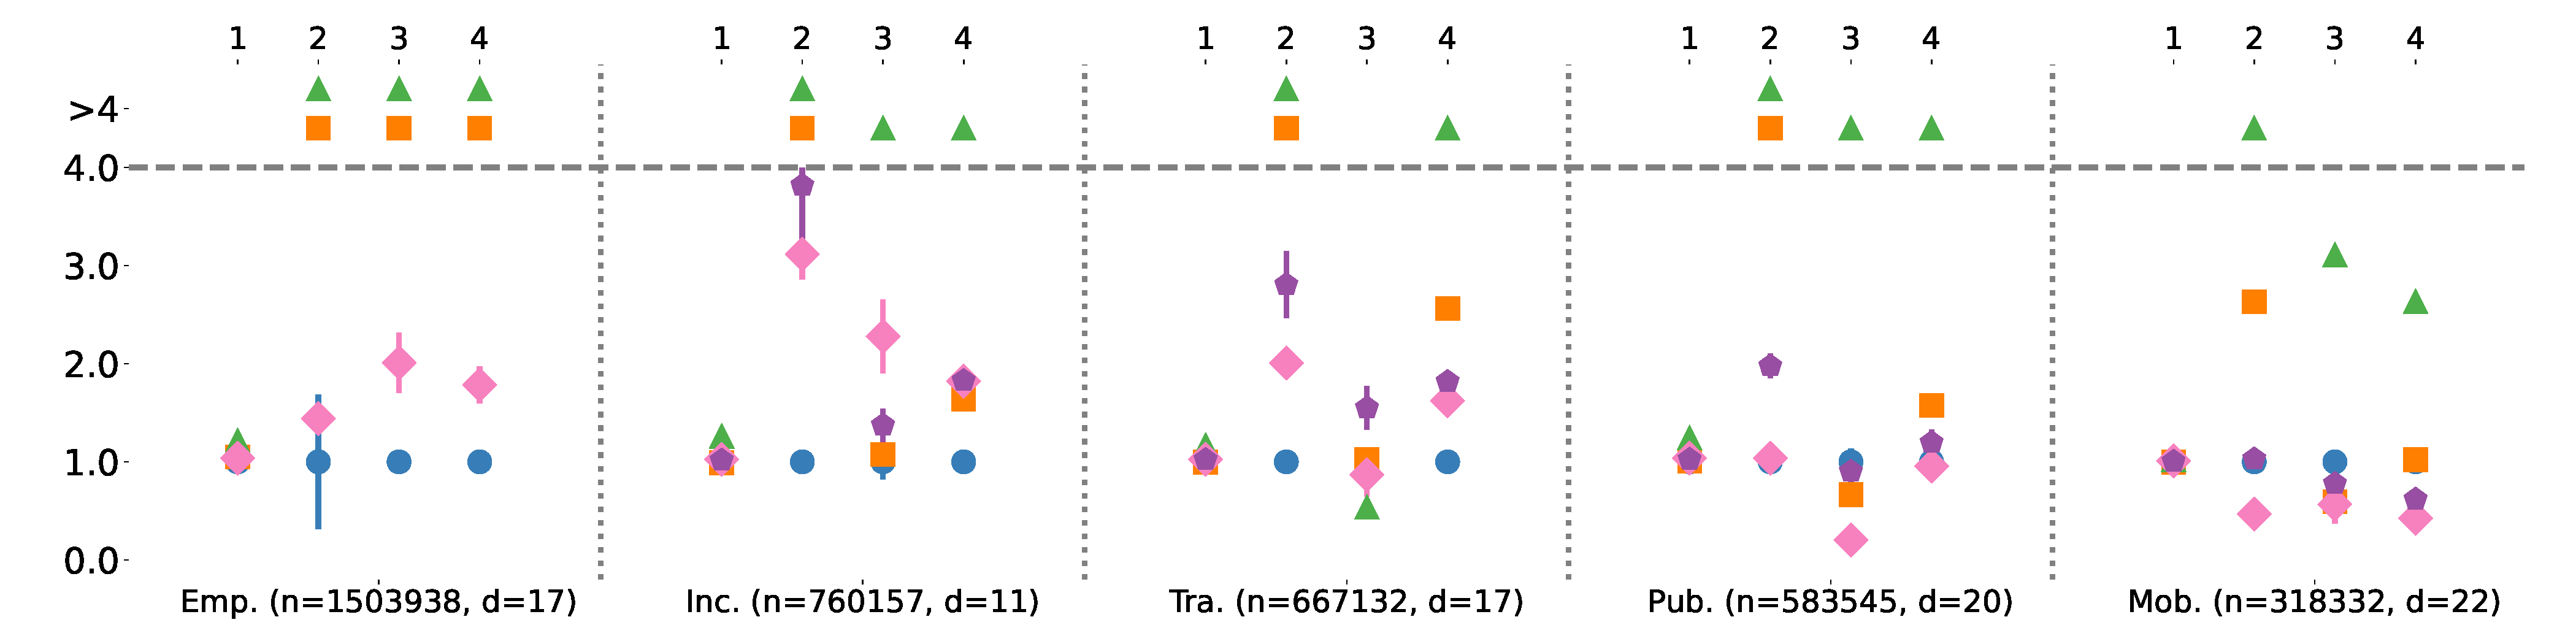
\includegraphics[width=0.9\textwidth]{papers/PrivPGD/figures/plots_datasets/eps_1.0/1.pdf}\\[1ex]
  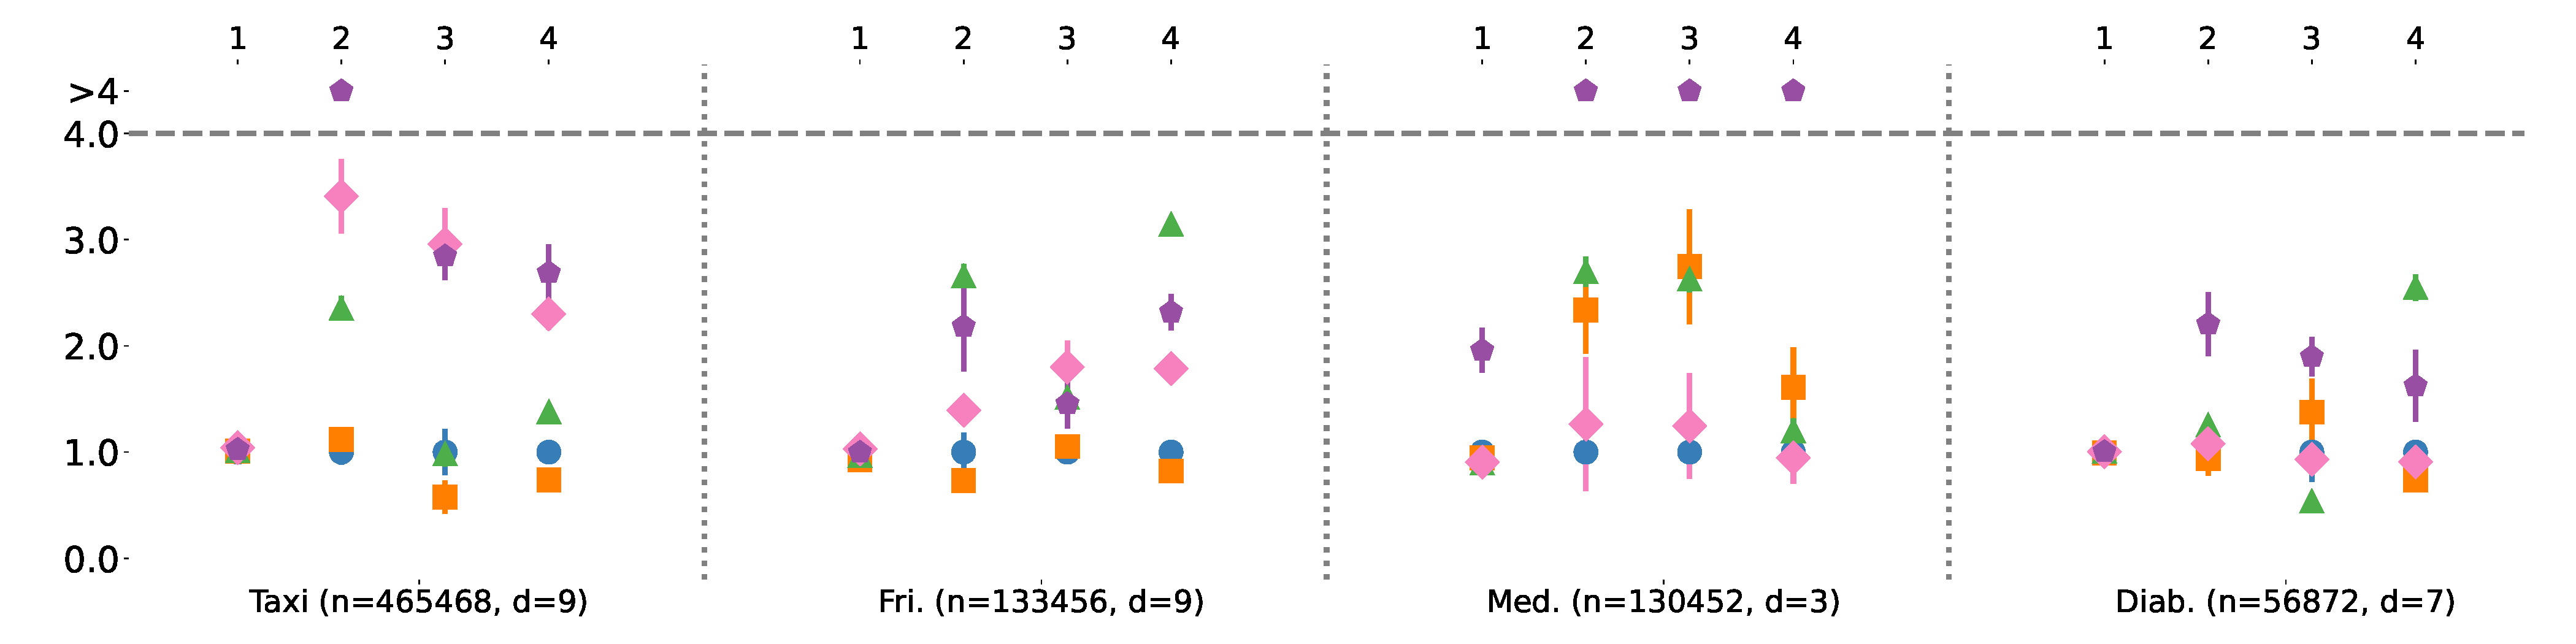
\includegraphics[width=0.9\textwidth]{papers/PrivPGD/figures/plots_datasets/eps_1.0/2.pdf}
  \caption{Extended benchmark comparison at \(\epsilon = 1.0\) and \(\delta = 10^{-5}\). Following Figure~\ref{fig:comp}, x-axis labels denote 1) downstream error, 2) covariance error, 3) threshold query error, and 4) counting query error, and each point reports the five-run mean and standard deviation of the linear error ratio relative to PrivPGD (PrivPGD equals \(1.0\), lower is better), with values above \(4.0\) stacked in order above the dashed line. GEM is omitted from the plots and reported in Tables~\ref{tab:app-privpgd-e10-acs} and \ref{tab:app-privpgd-e10-rest}.}
  \label{fig:app-privpgd-comp-1}
\end{figure}

\begin{figure}[!tbp]
  \centering
  
\includegraphics[width=0.9\textwidth]{papers/PrivPGD/figures/exp12legend_plot.pdf}\\[1ex]
  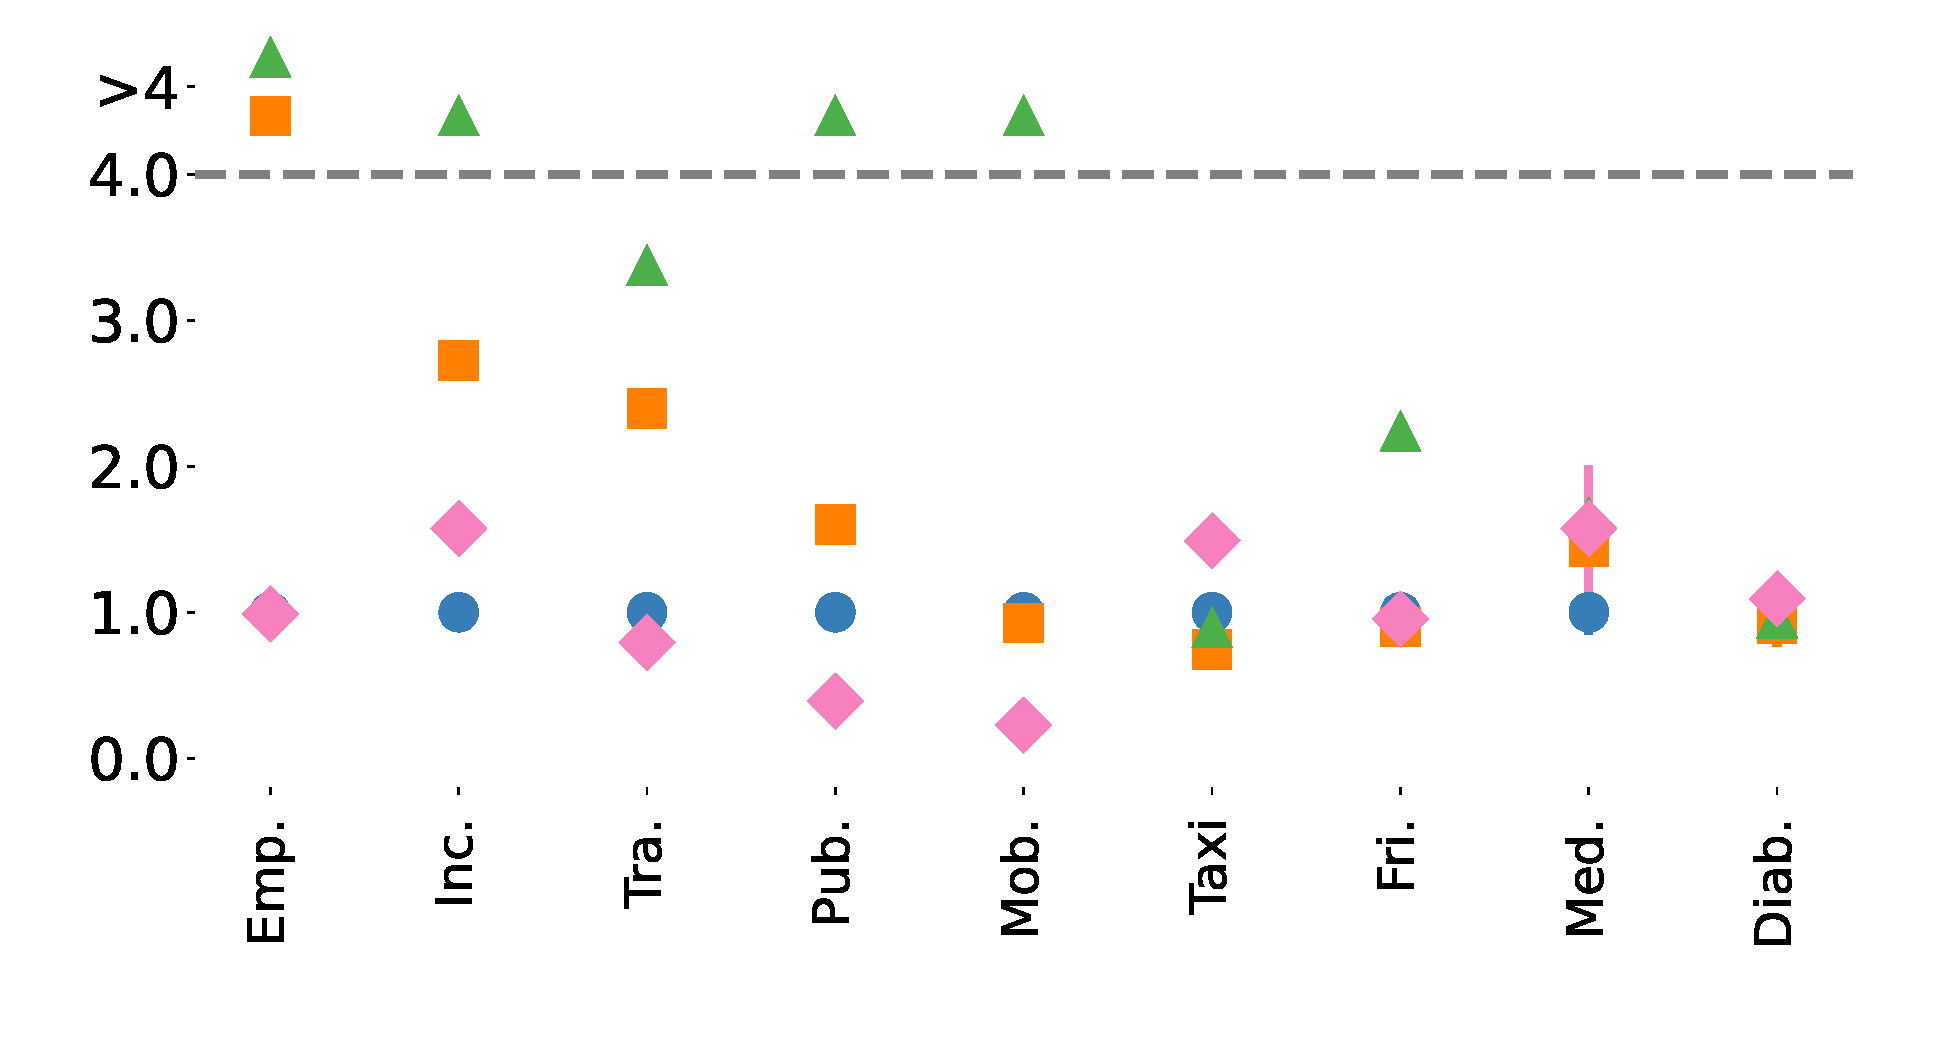
\includegraphics[width=0.48\textwidth]{papers/PrivPGD/figures/plots_distances/eps_1.0/wdist_1_2Way_avg.pdf}
  \hfill
  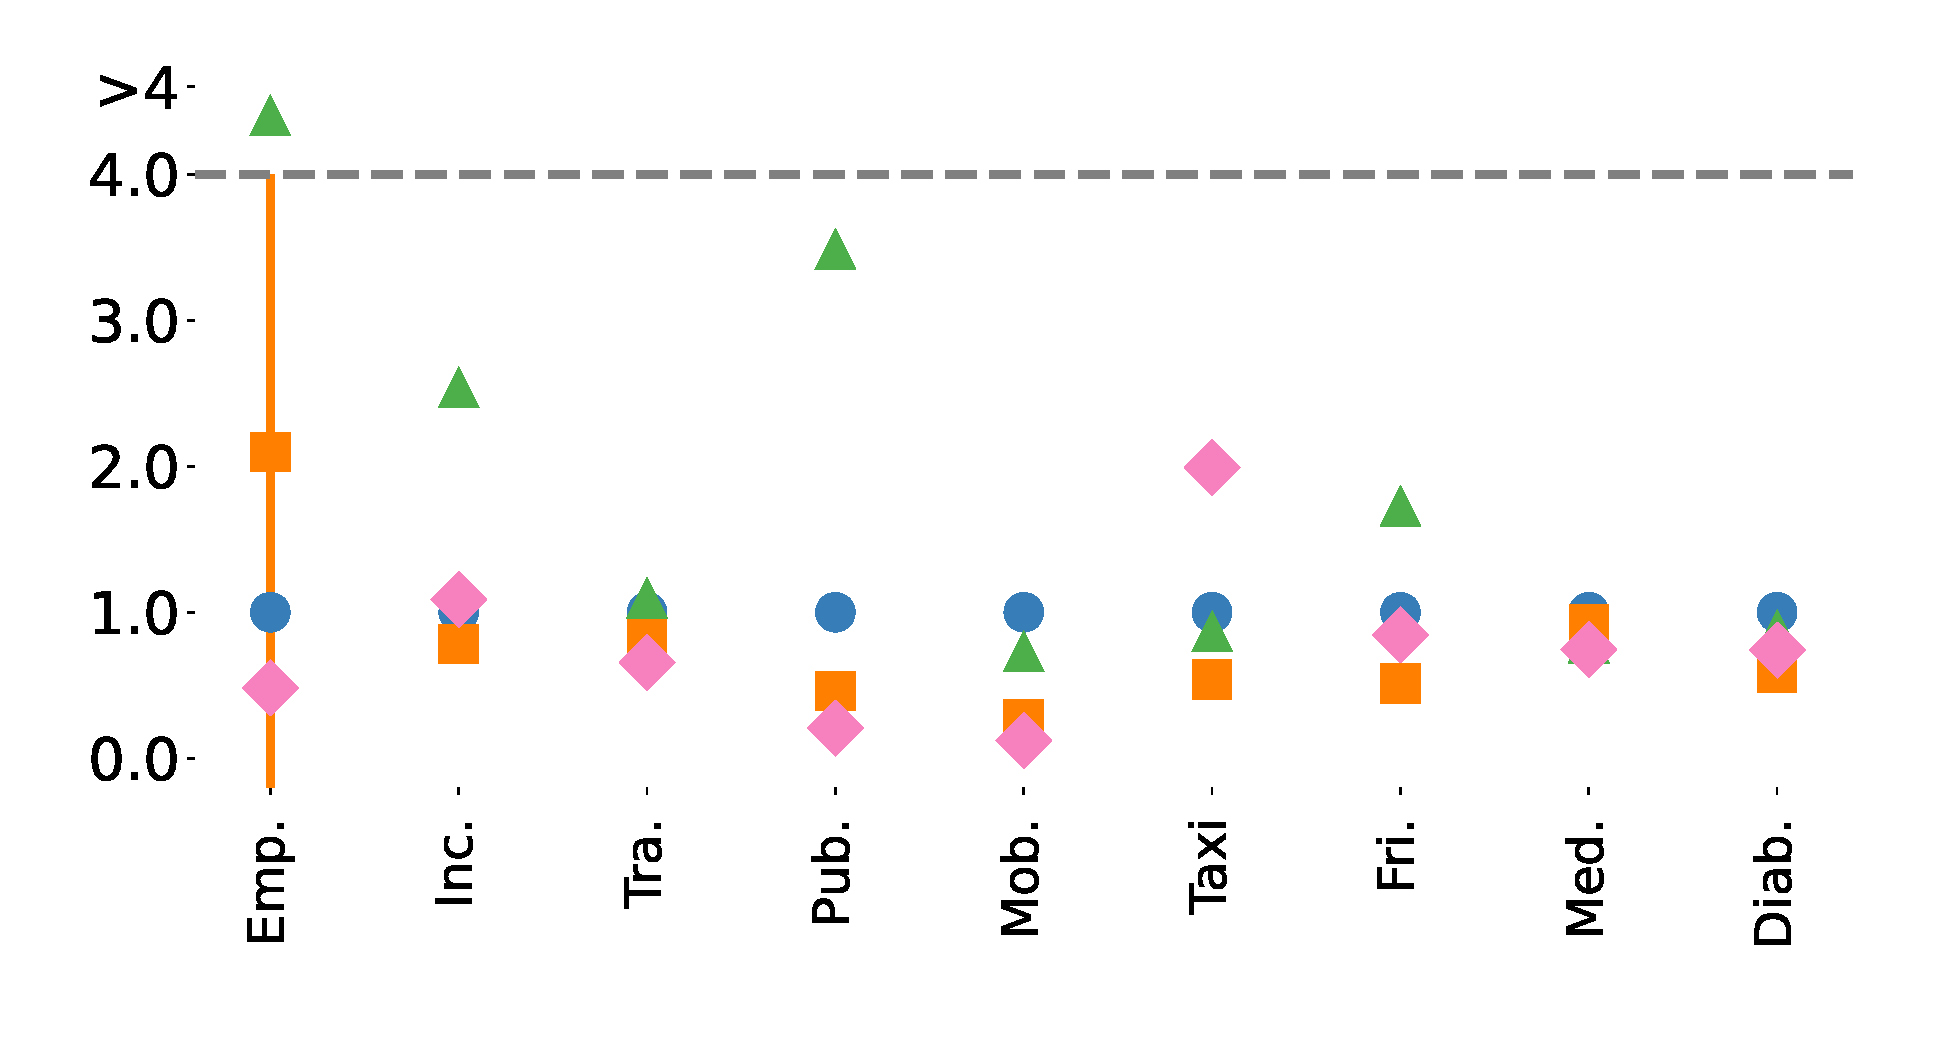
\includegraphics[width=0.48\textwidth]{papers/PrivPGD/figures/plots_distances/eps_1.0/newl1_2Way_avg.pdf}
  \caption{Average sliced Wasserstein distance (left) and average total variation distance (right) over all two-way marginals at \(\epsilon = 1.0\) and \(\delta = 10^{-5}\). Each point shows the five-run mean and standard deviation of the linear error ratio relative to PrivPGD (PrivPGD equals \(1.0\), lower is better), with values above \(4.0\) stacked in order above the dashed line. Only PrivPGD, PGM+AIM, PGM+MST, and Private GSD are plotted, and full results appear in Tables~\ref{tab:app-privpgd-e10-acs} and \ref{tab:app-privpgd-e10-rest}.}
  \label{fig:app-privpgd-dist-1}
\end{figure}

\FloatBarrier

\subsection{\texorpdfstring{$\epsilon = 0.2$}{epsilon = 0.2}}

At \(\epsilon = 0.2\) (Figures~\ref{fig:app-privpgd-comp-02} and \ref{fig:app-privpgd-dist-02}), the same trend becomes more pronounced. PGM+AIM, PGM+MST, and Private GSD more frequently outperform PrivPGD on query- and covariance-based metrics, especially when the data are smaller or higher-dimensional. The method nevertheless remains viable on several datasets, and the geometry-aware comparison still shows the expected advantage in sliced Wasserstein distance relative to total variation.

\begin{figure}[!tbp]
  \centering
  
\includegraphics[width=0.9\textwidth]{papers/PrivPGD/figures/exp12legend_plot.pdf}\\[1ex]
  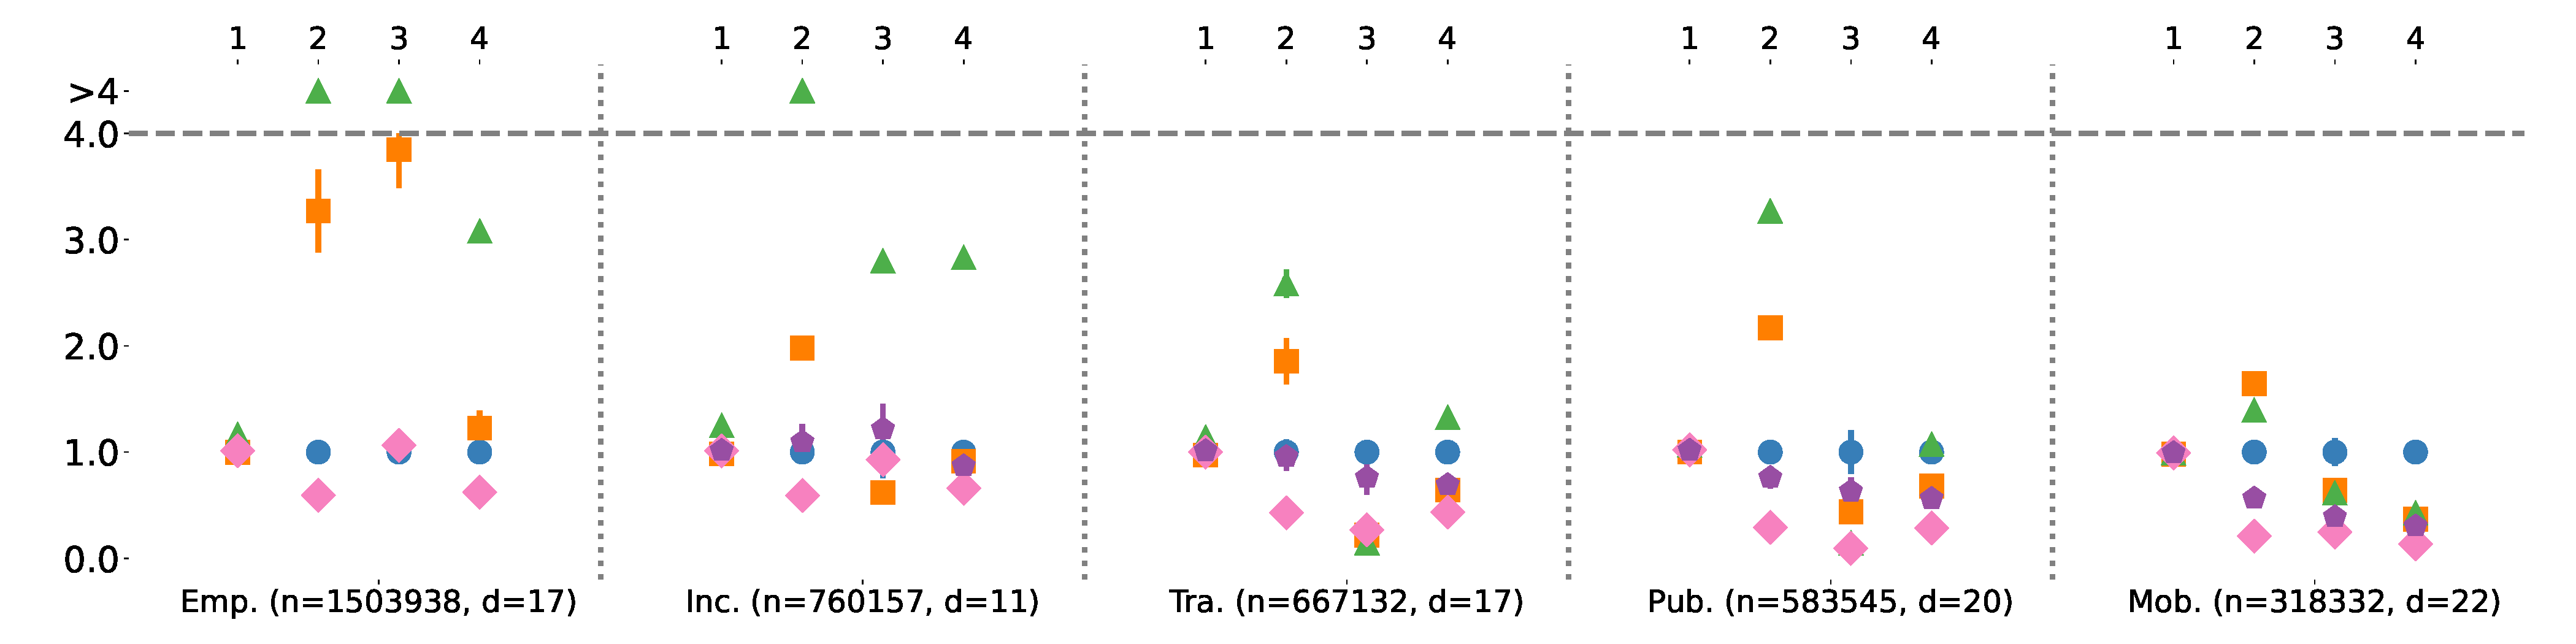
\includegraphics[width=0.9\textwidth]{papers/PrivPGD/figures/plots_datasets/eps_0.2/1.pdf}\\[1ex]
  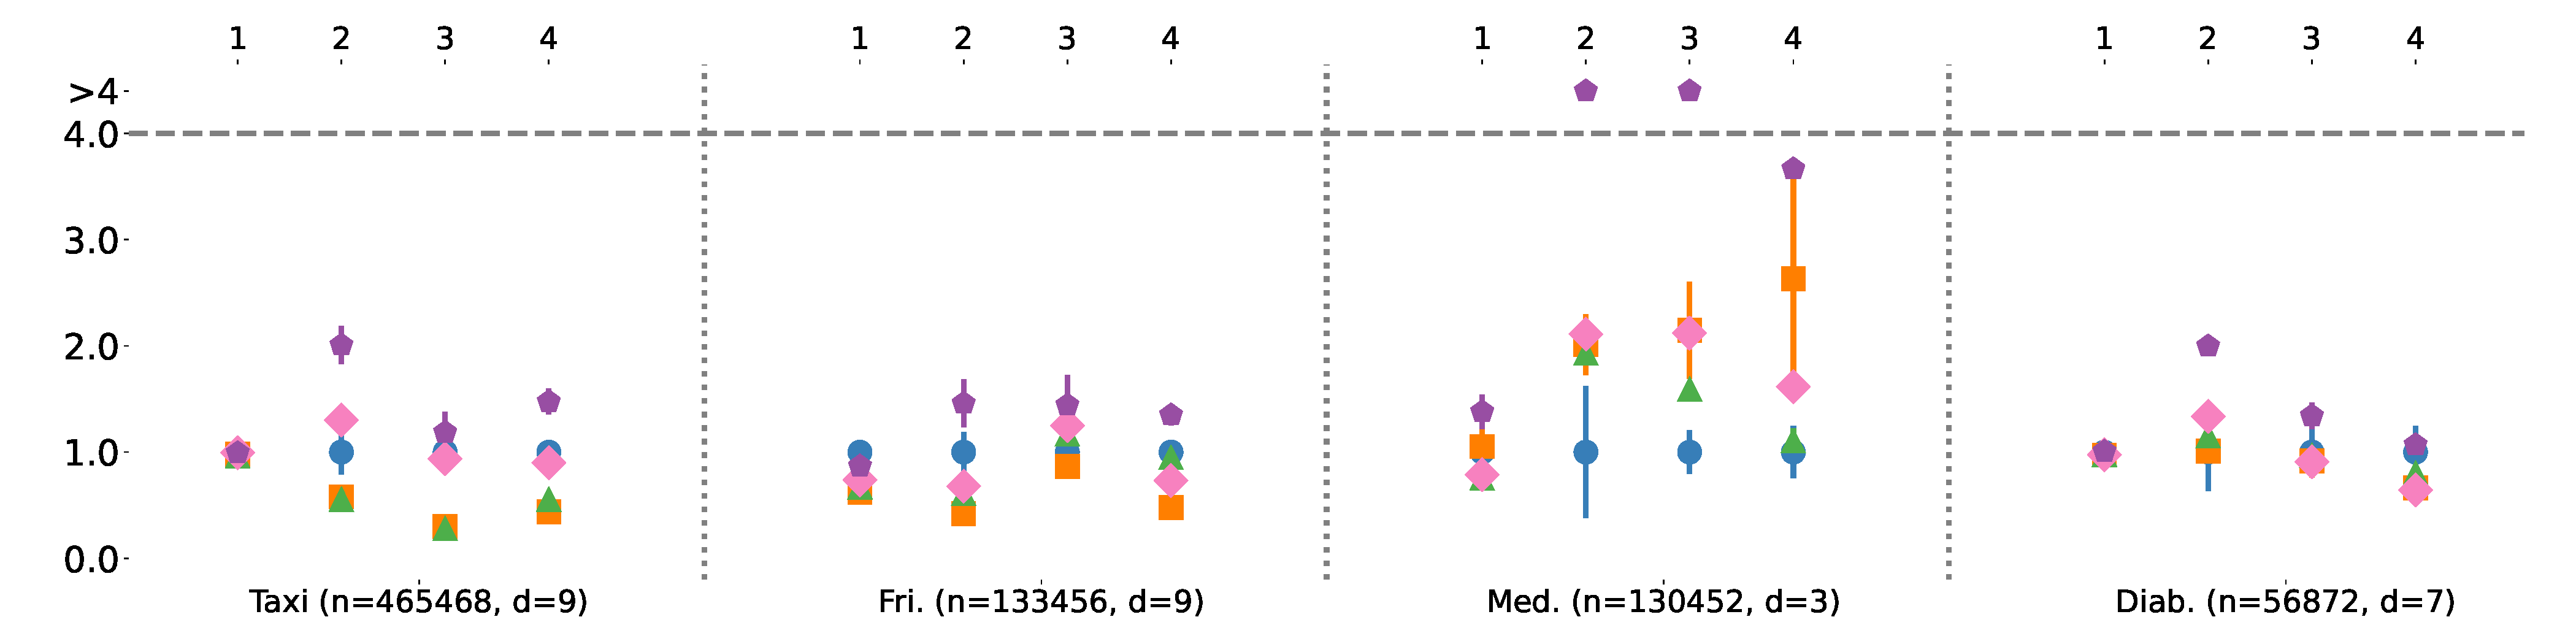
\includegraphics[width=0.9\textwidth]{papers/PrivPGD/figures/plots_datasets/eps_0.2/2.pdf}
  \caption{Extended benchmark comparison at \(\epsilon = 0.2\) and \(\delta = 10^{-5}\). Following Figure~\ref{fig:comp}, x-axis labels denote 1) downstream error, 2) covariance error, 3) threshold query error, and 4) counting query error, and each point reports the five-run mean and standard deviation of the linear error ratio relative to PrivPGD (PrivPGD equals \(1.0\), lower is better), with values above \(4.0\) stacked in order above the dashed line. GEM is omitted from the plots and reported in Tables~\ref{tab:app-privpgd-e02-acs} and \ref{tab:app-privpgd-e02-rest}.}
  \label{fig:app-privpgd-comp-02}
\end{figure}

\begin{figure}[!tbp]
  \centering
  
\includegraphics[width=0.9\textwidth]{papers/PrivPGD/figures/exp12legend_plot.pdf}\\[1ex]
  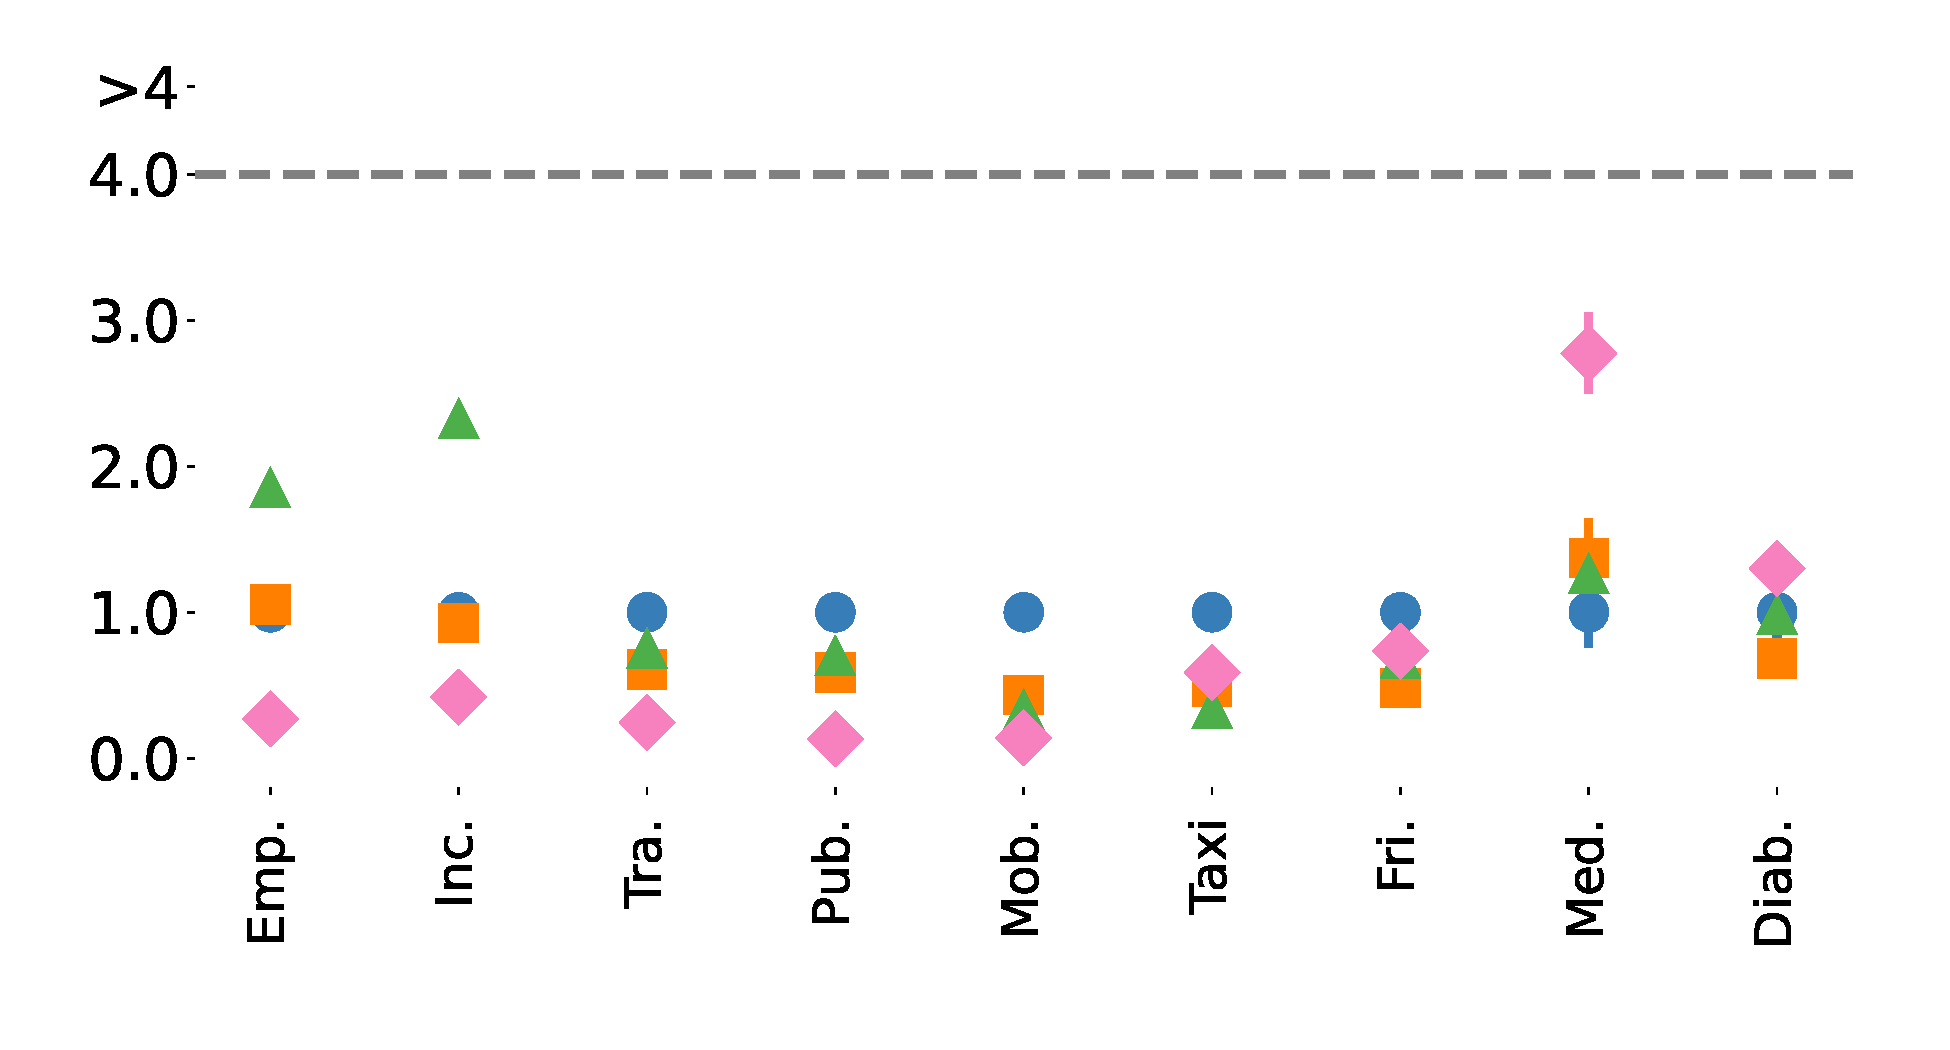
\includegraphics[width=0.48\textwidth]{papers/PrivPGD/figures/plots_distances/eps_0.2/wdist_1_2Way_avg.pdf}
  \hfill
  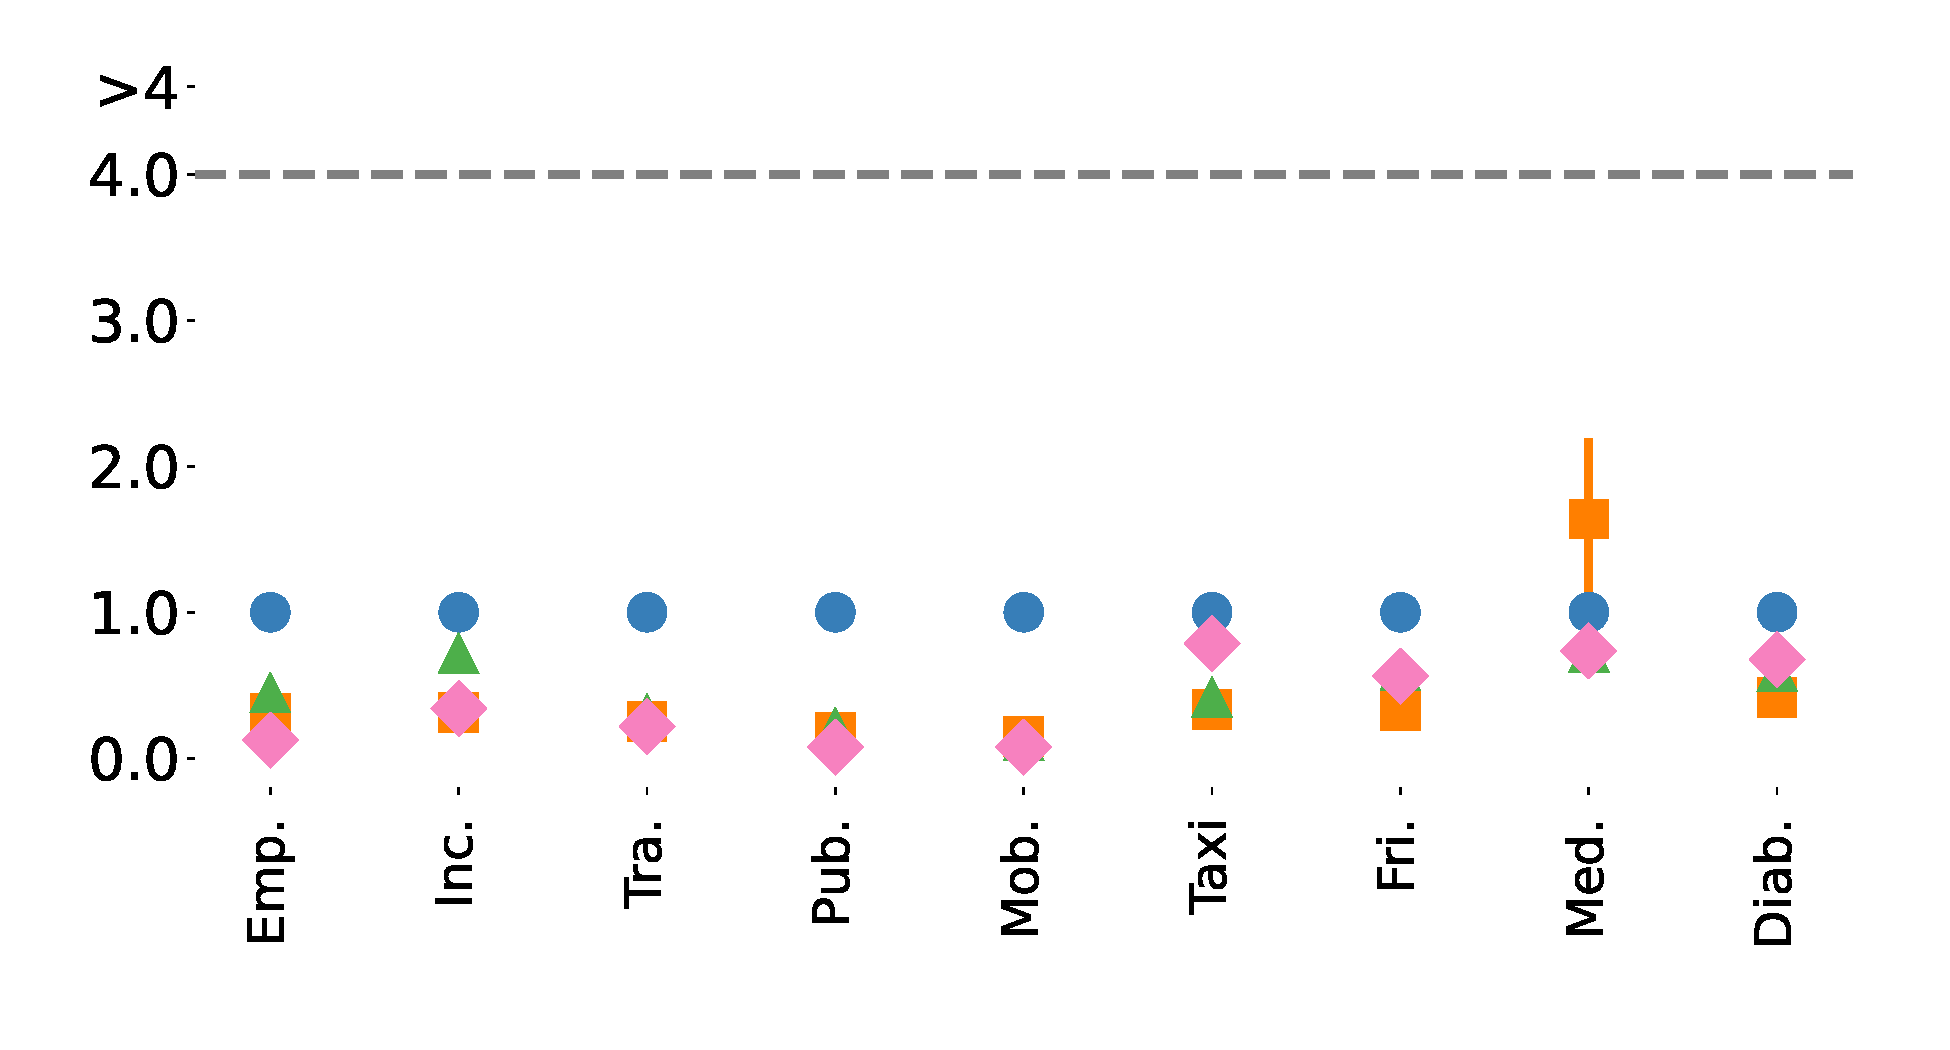
\includegraphics[width=0.48\textwidth]{papers/PrivPGD/figures/plots_distances/eps_0.2/newl1_2Way_avg.pdf}
  \caption{Average sliced Wasserstein distance (left) and average total variation distance (right) over all two-way marginals at \(\epsilon = 0.2\) and \(\delta = 10^{-5}\). Each point shows the five-run mean and standard deviation of the linear error ratio relative to PrivPGD (PrivPGD equals \(1.0\), lower is better), with values above \(4.0\) stacked in order above the dashed line. Only PrivPGD, PGM+AIM, PGM+MST, and Private GSD are plotted, and full results appear in Tables~\ref{tab:app-privpgd-e02-acs} and \ref{tab:app-privpgd-e02-rest}.}
  \label{fig:app-privpgd-dist-02}
\end{figure}

\FloatBarrier

\clearpage
\section{Detailed Benchmark Results}
\label{app:privpgd-tables}

The following tables report mean values over five runs, with the lowest error for each dataset and metric highlighted in bold. In the downstream column, the first number is the test error (0-1 error for classification and mean squared error for regression) of the model trained on the synthetic data, while the second number is the corresponding test error when the same model is trained on the original sensitive dataset. GEM and RAP are omitted on Emp. because they exceed the \(20\) GB memory budget.

\subsection{Primary Privacy Setting (\texorpdfstring{$\epsilon = 2.5$}{epsilon = 2.5})}

Tables~\ref{tab:app-privpgd-e25-acs} and \ref{tab:app-privpgd-e25-rest} collect the full benchmark results at the default privacy budget, separated into the ACS datasets and the remaining benchmarks.

\begin{table}[!tbp]
  \centering
  \scriptsize
  \resizebox{\textwidth}{!}{
  \begin{tabular}{llrrrrrr}
    \toprule
    Dataset & Method & Downstream & Covariance & Counting Query & Threshold Query & \(\SW_1\) & \(\TV\) \\
    \midrule
    Emp. & PrivPGD & \textbf{0.19}/0.19 & 0.02 & \textbf{0.00087} & \textbf{0.00043} & \textbf{0.00054} & 0.021 \\
    Emp. & PGM+AIM & \textbf{0.19}/0.19 & 0.04 & 0.0025 & 0.0026 & 0.0019 & 0.026 \\
    Emp. & PGM+MST & 0.33/0.19 & 0.27 & 0.012 & 0.0075 & 0.0087 & 0.10 \\
    Emp. & Private GSD & 0.20/0.19 & \textbf{0.0083} & 0.0013 & 0.00073 & 0.00059 & \textbf{0.013} \\
    \midrule
    Inc. & PrivPGD & \textbf{0.19}/0.19 & \textbf{0.0010} & \textbf{0.00078} & \textbf{0.00031} & \textbf{0.00043} & \textbf{0.028} \\
    Inc. & PGM+AIM & \textbf{0.19}/0.19 & 0.014 & 0.0017 & 0.00034 & 0.0017 & 0.034 \\
    Inc. & PGM+MST & 0.24/0.19 & 0.051 & 0.0077 & 0.0024 & 0.0054 & 0.11 \\
    Inc. & Private GSD & 0.20/0.19 & 0.0049 & 0.0017 & 0.00083 & 0.00093 & 0.045 \\
    Inc. & GEM & 0.22/0.19 & 0.047 & 0.010 & 0.0038 & 0.0099 & 0.17 \\
    Inc. & RAP & 0.20/0.19 & 0.0078 & 0.0017 & 0.00056 & 0.0011 & 0.037 \\
    \midrule
    Tra. & PrivPGD & \textbf{0.37}/0.34 & \textbf{0.0026} & \textbf{0.00065} & \textbf{0.00014} & \textbf{0.00049} & \textbf{0.027} \\
    Tra. & PGM+AIM & \textbf{0.37}/0.34 & 0.037 & 0.0023 & 0.00031 & 0.0019 & 0.035 \\
    Tra. & PGM+MST & 0.46/0.34 & 0.091 & 0.0058 & 0.00032 & 0.0038 & 0.061 \\
    Tra. & Private GSD & 0.38/0.34 & 0.011 & 0.0017 & 0.00037 & 0.00072 & 0.033 \\
    Tra. & GEM & 0.40/0.34 & 0.048 & 0.0052 & 0.0011 & 0.0041 & 0.076 \\
    Tra. & RAP & 0.38/0.34 & 0.015 & 0.0019 & 0.00047 & 0.0014 & 0.036 \\
    \midrule
    Pub. & PrivPGD & \textbf{0.28}/0.27 & 0.06 & \textbf{0.00097} & 0.00033 & 0.00094 & 0.037 \\
    Pub. & PGM+AIM & 0.32/0.27 & 0.10 & 0.0051 & 0.0012 & 0.0042 & 0.048 \\
    Pub. & PGM+MST & 0.35/0.27 & 0.41 & 0.010 & 0.00074 & 0.0088 & 0.092 \\
    Pub. & Private GSD & 0.30/0.27 & \textbf{0.012} & 0.0016 & \textbf{0.00015} & \textbf{0.00057} & \textbf{0.013} \\
    Pub. & GEM & 0.29/0.27 & 0.035 & 0.0031 & 0.00042 & 0.0019 & 0.029 \\
    Pub. & RAP & 0.29/0.27 & 0.020 & 0.0015 & 0.00054 & 0.0012 & 0.020 \\
    \midrule
    Mob. & PrivPGD & \textbf{0.23}/0.22 & \textbf{0.0091} & 0.0014 & 0.00051 & 0.0011 & 0.056 \\
    Mob. & PGM+AIM & \textbf{0.23}/0.22 & 0.05 & 0.0029 & \textbf{0.00036} & 0.0025 & 0.035 \\
    Mob. & PGM+MST & 0.24/0.22 & 0.29 & 0.0088 & 0.0050 & 0.0095 & 0.096 \\
    Mob. & Private GSD & 0.24/0.22 & 0.0092 & \textbf{0.0013} & 0.00068 & \textbf{0.00055} & \textbf{0.015} \\
    Mob. & GEM & 0.24/0.22 & 0.063 & 0.0074 & 0.0022 & 0.0060 & 0.082 \\
    Mob. & RAP & \textbf{0.23}/0.22 & 0.016 & 0.0014 & 0.00066 & 0.0013 & 0.022 \\
    \bottomrule
  \end{tabular}}
  \caption{Detailed benchmark results for the ACS datasets at \(\epsilon = 2.5\) and \(\delta = 10^{-5}\). Values are five-run means, with bold marking the lowest error per dataset and metric. Downstream reports synthetic/original test error, and GEM and RAP are omitted on Emp. due to the \(20\) GB memory limit.}
  \label{tab:app-privpgd-e25-acs}
\end{table}

\begin{table}[!tbp]
  \centering
  \scriptsize
  \resizebox{\textwidth}{!}{
  \begin{tabular}{llrrrrrr}
    \toprule
    Dataset & Method & Downstream & Covariance & Counting Query & Threshold Query & \(\SW_1\) & \(\TV\) \\
    \midrule
    Taxi & PrivPGD & \textbf{2.3}/2.2 & \textbf{0.00048} & \textbf{0.00051} & \textbf{0.00011} & \textbf{0.00027} & 0.020 \\
    Taxi & PGM+AIM & \textbf{2.3}/2.2 & 0.0013 & 0.00066 & \textbf{0.00011} & 0.00050 & \textbf{0.016} \\
    Taxi & PGM+MST & \textbf{2.3}/2.2 & 0.0029 & 0.0011 & 0.00020 & 0.00058 & 0.028 \\
    Taxi & Private GSD & \textbf{2.3}/2.2 & 0.0040 & 0.0019 & 0.00061 & 0.00093 & 0.064 \\
    Taxi & GEM & 2.7/2.2 & 0.079 & 0.016 & 0.0037 & 0.018 & 0.36 \\
    Taxi & RAP & \textbf{2.3}/2.2 & 0.0065 & 0.0021 & 0.00050 & 0.0013 & 0.078 \\
    \midrule
    Fri. & PrivPGD & \textbf{1.5}/1.4 & \textbf{0.00097} & \textbf{0.00064} & \textbf{0.00053} & \textbf{0.00033} & 0.015 \\
    Fri. & PGM+AIM & \textbf{1.5}/1.4 & 0.0014 & \textbf{0.00064} & 0.00058 & 0.00054 & \textbf{0.011} \\
    Fri. & PGM+MST & \textbf{1.5}/1.4 & 0.0057 & 0.0027 & 0.00080 & 0.0014 & 0.047 \\
    Fri. & Private GSD & 1.7/1.4 & 0.0032 & 0.0015 & 0.00083 & 0.00060 & 0.021 \\
    Fri. & GEM & 2.8/1.4 & 0.031 & 0.0066 & 0.0016 & 0.0090 & 0.16 \\
    Fri. & RAP & \textbf{1.5}/1.4 & 0.0038 & 0.0018 & 0.00075 & 0.0011 & 0.034 \\
    \midrule
    Med. & PrivPGD & 2.2/2.1 & 0.00014 & \textbf{0.0012} & \textbf{0.00013} & \textbf{0.00036} & 0.023 \\
    Med. & PGM+AIM & \textbf{2.1}/2.1 & 0.00066 & \textbf{0.0012} & 0.00034 & 0.00076 & \textbf{0.013} \\
    Med. & PGM+MST & \textbf{2.1}/2.1 & 0.00061 & \textbf{0.0012} & 0.00035 & 0.00070 & 0.017 \\
    Med. & Private GSD & 2.2/2.1 & \textbf{0.00013} & \textbf{0.0012} & 0.00014 & 0.00076 & 0.020 \\
    Med. & GEM & 75/2.1 & 0.11 & 0.10 & 0.054 & 0.22 & 1.4 \\
    Med. & RAP & 4.5/2.1 & 0.0048 & 0.013 & 0.0023 & 0.0070 & 0.062 \\
    \midrule
    Diab. & PrivPGD & \textbf{0.4}/0.4 & \textbf{0.0013} & \textbf{0.0013} & 0.00042 & 0.00084 & 0.028 \\
    Diab. & PGM+AIM & \textbf{0.4}/0.4 & 0.0045 & 0.0025 & 0.0015 & 0.0022 & 0.028 \\
    Diab. & PGM+MST & 0.41/0.4 & 0.0047 & 0.0083 & 0.00029 & 0.0017 & 0.045 \\
    Diab. & Private GSD & 0.41/0.4 & 0.0017 & 0.0017 & \textbf{0.00026} & \textbf{0.00067} & \textbf{0.026} \\
    Diab. & GEM & 0.41/0.4 & 0.042 & 0.032 & 0.0084 & 0.032 & 0.23 \\
    Diab. & RAP & 0.41/0.4 & 0.0034 & 0.0021 & 0.00097 & 0.0025 & 0.041 \\
    \bottomrule
  \end{tabular}}
  \caption{Detailed benchmark results for the remaining datasets at \(\epsilon = 2.5\) and \(\delta = 10^{-5}\). Values are five-run means, with bold marking the lowest error per dataset and metric. Downstream reports synthetic/original test error.}
  \label{tab:app-privpgd-e25-rest}
\end{table}

\clearpage
\subsection{Lower Budget (\texorpdfstring{$\epsilon = 1.0$}{epsilon = 1.0})}

Tables~\ref{tab:app-privpgd-e10-acs} and \ref{tab:app-privpgd-e10-rest} report the same benchmark split at \(\epsilon = 1.0\), where the relative gap between PrivPGD and the strongest baselines narrows.

\begin{table}[!tbp]
  \centering
  \scriptsize
  \resizebox{\textwidth}{!}{
  \begin{tabular}{llrrrrrr}
    \toprule
    Dataset & Method & Downstream & Covariance & Counting Query & Threshold Query & \(\SW_1\) & \(\TV\) \\
    \midrule
    Emp. & PrivPGD & \textbf{0.19}/0.19 & \textbf{0.0056} & \textbf{0.00077} & \textbf{0.00038} & 0.00060 & 0.027 \\
    Emp. & PGM+AIM & 0.20/0.19 & 0.063 & 0.0036 & 0.0040 & 0.0042 & 0.057 \\
    Emp. & PGM+MST & 0.23/0.19 & 0.48 & 0.098 & 0.081 & 0.14 & 0.70 \\
    Emp. & Private GSD & 0.20/0.19 & 0.0080 & 0.0014 & 0.00076 & \textbf{0.00059} & \textbf{0.013} \\
    \midrule
    Inc. & PrivPGD & \textbf{0.19}/0.19 & \textbf{0.0019} & \textbf{0.00092} & \textbf{0.00039} & \textbf{0.00060} & 0.042 \\
    Inc. & PGM+AIM & \textbf{0.19}/0.19 & 0.014 & 0.0015 & 0.00042 & 0.0016 & \textbf{0.033} \\
    Inc. & PGM+MST & 0.24/0.19 & 0.052 & 0.0077 & 0.0024 & 0.0054 & 0.11 \\
    Inc. & Private GSD & 0.20/0.19 & 0.0061 & 0.0017 & 0.00089 & 0.00095 & 0.046 \\
    Inc. & GEM & 0.22/0.19 & 0.047 & 0.010 & 0.0037 & 0.0098 & 0.16 \\
    Inc. & RAP & \textbf{0.19}/0.19 & 0.0074 & 0.0017 & 0.00054 & 0.0010 & 0.041 \\
    \midrule
    Tra. & PrivPGD & \textbf{0.37}/0.34 & \textbf{0.0055} & \textbf{0.0011} & 0.00032 & 0.00091 & 0.050 \\
    Tra. & PGM+AIM & \textbf{0.37}/0.34 & 0.036 & 0.0027 & 0.00033 & 0.0022 & 0.042 \\
    Tra. & PGM+MST & 0.44/0.34 & 0.073 & 0.0058 & \textbf{0.00017} & 0.0031 & 0.055 \\
    Tra. & Private GSD & 0.38/0.34 & 0.011 & 0.0017 & 0.00028 & \textbf{0.00072} & \textbf{0.033} \\
    Tra. & GEM & 0.40/0.34 & 0.048 & 0.0051 & 0.00091 & 0.0040 & 0.074 \\
    Tra. & RAP & 0.38/0.34 & 0.016 & 0.0019 & 0.00050 & 0.0016 & 0.041 \\
    \midrule
    Pub. & PrivPGD & \textbf{0.28}/0.27 & \textbf{0.011} & 0.0015 & 0.00061 & 0.0014 & 0.061 \\
    Pub. & PGM+AIM & \textbf{0.28}/0.27 & 0.058 & 0.0024 & 0.00041 & 0.0023 & 0.028 \\
    Pub. & PGM+MST & 0.35/0.27 & 0.29 & 0.024 & 0.0092 & 0.040 & 0.21 \\
    Pub. & Private GSD & 0.29/0.27 & 0.012 & \textbf{0.0014} & \textbf{0.00012} & \textbf{0.00055} & \textbf{0.013} \\
    Pub. & GEM & 0.29/0.27 & 0.031 & 0.0029 & 0.00056 & 0.0017 & 0.025 \\
    Pub. & RAP & 0.29/0.27 & 0.022 & 0.0018 & 0.00055 & 0.0014 & 0.023 \\
    \midrule
    Mob. & PrivPGD & \textbf{0.23}/0.22 & 0.021 & 0.0029 & 0.00085 & 0.0026 & 0.13 \\
    Mob. & PGM+AIM & \textbf{0.23}/0.22 & 0.054 & 0.0028 & 0.00051 & 0.0024 & 0.034 \\
    Mob. & PGM+MST & 0.24/0.22 & 0.13 & 0.0077 & 0.0027 & 0.013 & 0.093 \\
    Mob. & Private GSD & 0.24/0.22 & \textbf{0.0096} & \textbf{0.0012} & \textbf{0.00049} & \textbf{0.00060} & \textbf{0.016} \\
    Mob. & GEM & 0.24/0.22 & 0.062 & 0.0077 & 0.0021 & 0.0062 & 0.083 \\
    Mob. & RAP & \textbf{0.23}/0.22 & 0.021 & 0.0018 & 0.00066 & 0.0017 & 0.031 \\
    \bottomrule
  \end{tabular}}
  \caption{Detailed benchmark results for the ACS datasets at \(\epsilon = 1.0\) and \(\delta = 10^{-5}\). Values are five-run means, with bold marking the lowest error per dataset and metric. Downstream reports synthetic/original test error, and GEM and RAP are omitted on Emp. due to the \(20\) GB memory limit.}
  \label{tab:app-privpgd-e10-acs}
\end{table}

\begin{table}[!tbp]
  \centering
  \scriptsize
  \resizebox{\textwidth}{!}{
  \begin{tabular}{llrrrrrr}
    \toprule
    Dataset & Method & Downstream & Covariance & Counting Query & Threshold Query & \(\SW_1\) & \(\TV\) \\
    \midrule
    Taxi & PrivPGD & \textbf{2.3}/2.2 & \textbf{0.0013} & 0.00077 & 0.00018 & 0.00062 & 0.033 \\
    Taxi & PGM+AIM & \textbf{2.3}/2.2 & 0.0014 & \textbf{0.00057} & \textbf{0.00011} & \textbf{0.00046} & \textbf{0.018} \\
    Taxi & PGM+MST & \textbf{2.3}/2.2 & 0.0030 & 0.0011 & 0.00018 & 0.00055 & 0.029 \\
    Taxi & Private GSD & 2.4/2.2 & 0.0043 & 0.0018 & 0.00055 & 0.00092 & 0.066 \\
    Taxi & GEM & 2.8/2.2 & 0.081 & 0.017 & 0.0045 & 0.021 & 0.36 \\
    Taxi & RAP & \textbf{2.3}/2.2 & 0.0061 & 0.0021 & 0.00052 & 0.0014 & 0.080 \\
    \midrule
    Fri. & PrivPGD & 1.6/1.4 & 0.0022 & 0.00086 & \textbf{0.00053} & 0.00068 & 0.028 \\
    Fri. & PGM+AIM & \textbf{1.5}/1.4 & \textbf{0.0016} & \textbf{0.00071} & 0.00056 & \textbf{0.00061} & \textbf{0.014} \\
    Fri. & PGM+MST & \textbf{1.5}/1.4 & 0.0058 & 0.0027 & 0.00081 & 0.0015 & 0.049 \\
    Fri. & Private GSD & 1.6/1.4 & 0.0031 & 0.0015 & 0.00096 & 0.00065 & 0.024 \\
    Fri. & GEM & 2.8/1.4 & 0.031 & 0.0068 & 0.0014 & 0.0092 & 0.16 \\
    Fri. & RAP & 1.6/1.4 & 0.0048 & 0.0020 & 0.00078 & 0.0016 & 0.046 \\
    \midrule
    Med. & PrivPGD & 2.4/2.1 & \textbf{0.00032} & 0.0015 & \textbf{0.00019} & \textbf{0.00061} & 0.030 \\
    Med. & PGM+AIM & 2.3/2.1 & 0.00076 & 0.0024 & 0.00053 & 0.00088 & 0.027 \\
    Med. & PGM+MST & \textbf{2.1}/2.1 & 0.00088 & 0.0018 & 0.00051 & 0.0010 & 0.023 \\
    Med. & Private GSD & 2.2/2.1 & 0.00041 & \textbf{0.0014} & 0.00024 & 0.00095 & \textbf{0.022} \\
    Med. & GEM & 75/2.1 & 0.11 & 0.10 & 0.054 & 0.22 & 1.4 \\
    Med. & RAP & 4.7/2.1 & 0.0051 & 0.013 & 0.0024 & 0.0070 & 0.066 \\
    \midrule
    Diab. & PrivPGD & \textbf{0.4}/0.4 & 0.0033 & 0.0026 & 0.0010 & 0.0020 & 0.052 \\
    Diab. & PGM+AIM & \textbf{0.4}/0.4 & \textbf{0.0031} & \textbf{0.0019} & 0.0014 & \textbf{0.0019} & \textbf{0.030} \\
    Diab. & PGM+MST & 0.41/0.4 & 0.0042 & 0.0067 & \textbf{0.00056} & \textbf{0.0019} & 0.045 \\
    Diab. & Private GSD & 0.41/0.4 & 0.0036 & 0.0024 & 0.00096 & 0.0022 & 0.039 \\
    Diab. & GEM & 0.41/0.4 & 0.040 & 0.031 & 0.0078 & 0.030 & 0.22 \\
    Diab. & RAP & 0.41/0.4 & 0.0073 & 0.0043 & 0.0020 & 0.0054 & 0.071 \\
    \bottomrule
  \end{tabular}}
  \caption{Detailed benchmark results for the remaining datasets at \(\epsilon = 1.0\) and \(\delta = 10^{-5}\). Values are five-run means, with bold marking the lowest error per dataset and metric. Downstream reports synthetic/original test error.}
  \label{tab:app-privpgd-e10-rest}
\end{table}

\clearpage
\subsection{Lower Budget (\texorpdfstring{$\epsilon = 0.2$}{epsilon = 0.2})}

Tables~\ref{tab:app-privpgd-e02-acs} and \ref{tab:app-privpgd-e02-rest} summarize the highest-noise setting, which makes the appendix's lower-budget discussion concrete at the full table level.

\begin{table}[!tbp]
  \centering
  \scriptsize
  \resizebox{\textwidth}{!}{
  \begin{tabular}{llrrrrrr}
    \toprule
    Dataset & Method & Downstream & Covariance & Counting Query & Threshold Query & \(\SW_1\) & \(\TV\) \\
    \midrule
    Emp. & PrivPGD & \textbf{0.19}/0.19 & 0.015 & 0.0022 & \textbf{0.00078} & 0.0023 & 0.11 \\
    Emp. & PGM+AIM & \textbf{0.19}/0.19 & 0.049 & 0.0027 & 0.0031 & 0.0024 & 0.035 \\
    Emp. & PGM+MST & 0.23/0.19 & 0.10 & 0.0067 & 0.0047 & 0.0043 & 0.050 \\
    Emp. & Private GSD & 0.20/0.19 & \textbf{0.0088} & \textbf{0.0014} & 0.00083 & \textbf{0.00063} & \textbf{0.014} \\
    \midrule
    Inc. & PrivPGD & \textbf{0.19}/0.19 & 0.0098 & 0.0027 & 0.00086 & 0.0024 & 0.15 \\
    Inc. & PGM+AIM & \textbf{0.19}/0.19 & 0.019 & 0.0025 & \textbf{0.00053} & 0.0022 & \textbf{0.048} \\
    Inc. & PGM+MST & 0.24/0.19 & 0.052 & 0.0077 & 0.0024 & 0.0056 & 0.11 \\
    Inc. & Private GSD & 0.20/0.19 & \textbf{0.0058} & \textbf{0.0018} & 0.00080 & \textbf{0.0010} & 0.052 \\
    Inc. & GEM & 0.22/0.19 & 0.046 & 0.0099 & 0.0035 & 0.0096 & 0.16 \\
    Inc. & RAP & 0.20/0.19 & 0.011 & 0.0024 & 0.0010 & 0.0019 & 0.072 \\
    \midrule
    Tra. & PrivPGD & 0.38/0.34 & 0.027 & 0.0043 & 0.0012 & 0.0040 & 0.19 \\
    Tra. & PGM+AIM & \textbf{0.37}/0.34 & 0.050 & 0.0028 & 0.00027 & 0.0024 & 0.048 \\
    Tra. & PGM+MST & 0.44/0.34 & 0.070 & 0.0058 & \textbf{0.00018} & 0.0030 & 0.057 \\
    Tra. & Private GSD & 0.38/0.34 & \textbf{0.012} & \textbf{0.0019} & 0.00033 & \textbf{0.00097} & \textbf{0.041} \\
    Tra. & GEM & 0.40/0.34 & 0.048 & 0.0051 & 0.00093 & 0.0040 & 0.073 \\
    Tra. & RAP & 0.39/0.34 & 0.026 & 0.0030 & 0.00093 & 0.0033 & 0.074 \\
    \midrule
    Pub. & PrivPGD & \textbf{0.29}/0.27 & 0.048 & 0.0058 & 0.0021 & 0.0064 & 0.24 \\
    Pub. & PGM+AIM & \textbf{0.29}/0.27 & 0.10 & 0.0039 & 0.00093 & 0.0037 & 0.043 \\
    Pub. & PGM+MST & 0.31/0.27 & 0.16 & 0.0062 & 0.00031 & 0.0045 & 0.050 \\
    Pub. & Private GSD & \textbf{0.29}/0.27 & \textbf{0.014} & \textbf{0.0017} & \textbf{0.00020} & \textbf{0.00085} & \textbf{0.019} \\
    Pub. & GEM & \textbf{0.29}/0.27 & 0.044 & 0.0039 & 0.00053 & 0.0025 & 0.035 \\
    Pub. & RAP & \textbf{0.29}/0.27 & 0.037 & 0.0033 & 0.0013 & 0.0030 & 0.049 \\
    \midrule
    Mob. & PrivPGD & 0.24/0.22 & 0.085 & 0.014 & 0.0030 & 0.011 & 0.46 \\
    Mob. & PGM+AIM & \textbf{0.23}/0.22 & 0.14 & 0.0052 & 0.0019 & 0.0049 & 0.068 \\
    Mob. & PGM+MST & 0.24/0.22 & 0.12 & 0.0060 & 0.0019 & 0.0037 & 0.054 \\
    Mob. & Private GSD & 0.24/0.22 & \textbf{0.018} & \textbf{0.0019} & \textbf{0.00076} & \textbf{0.0016} & \textbf{0.035} \\
    Mob. & GEM & 0.24/0.22 & 0.062 & 0.0076 & 0.0018 & 0.0058 & 0.078 \\
    Mob. & RAP & 0.24/0.22 & 0.048 & 0.0043 & 0.0012 & 0.0048 & 0.080 \\
    \bottomrule
  \end{tabular}}
  \caption{Detailed benchmark results for the ACS datasets at \(\epsilon = 0.2\) and \(\delta = 10^{-5}\). Values are five-run means, with bold marking the lowest error per dataset and metric. Downstream reports synthetic/original test error, and GEM and RAP are omitted on Emp. due to the \(20\) GB memory limit.}
  \label{tab:app-privpgd-e02-acs}
\end{table}

\begin{table}[!tbp]
  \centering
  \scriptsize
  \resizebox{\textwidth}{!}{
  \begin{tabular}{llrrrrrr}
    \toprule
    Dataset & Method & Downstream & Covariance & Counting Query & Threshold Query & \(\SW_1\) & \(\TV\) \\
    \midrule
    Taxi & PrivPGD & 2.4/2.2 & 0.0055 & 0.0025 & 0.00072 & 0.0026 & 0.11 \\
    Taxi & PGM+AIM & \textbf{2.3}/2.2 & 0.0032 & \textbf{0.0011} & 0.00022 & 0.0013 & \textbf{0.037} \\
    Taxi & PGM+MST & \textbf{2.3}/2.2 & \textbf{0.0030} & 0.0014 & \textbf{0.00020} & \textbf{0.00087} & 0.046 \\
    Taxi & Private GSD & 2.4/2.2 & 0.0071 & 0.0022 & 0.00068 & 0.0015 & 0.087 \\
    Taxi & GEM & 2.8/2.2 & 0.082 & 0.017 & 0.0042 & 0.020 & 0.36 \\
    Taxi & RAP & 2.4/2.2 & 0.011 & 0.0036 & 0.00086 & 0.0036 & 0.17 \\
    \midrule
    Fri. & PrivPGD & 2.5/1.4 & 0.011 & 0.0031 & 0.00071 & 0.0031 & 0.11 \\
    Fri. & PGM+AIM & \textbf{1.5}/1.4 & \textbf{0.0048} & \textbf{0.0015} & \textbf{0.00061} & \textbf{0.0015} & \textbf{0.036} \\
    Fri. & PGM+MST & 1.6/1.4 & 0.0069 & 0.0030 & 0.00082 & 0.0021 & 0.065 \\
    Fri. & Private GSD & 1.8/1.4 & 0.0077 & 0.0023 & 0.00088 & 0.0023 & 0.061 \\
    Fri. & GEM & 2.8/1.4 & 0.031 & 0.0065 & 0.0014 & 0.0083 & 0.15 \\
    Fri. & RAP & 2.1/1.4 & 0.017 & 0.0042 & 0.0010 & 0.0055 & 0.12 \\
    \midrule
    Med. & PrivPGD & 3.0/2.1 & \textbf{0.0013} & \textbf{0.0048} & \textbf{0.00082} & \textbf{0.0024} & 0.076 \\
    Med. & PGM+AIM & 3.1/2.1 & 0.0027 & 0.013 & 0.0018 & 0.0033 & 0.12 \\
    Med. & PGM+MST & \textbf{2.2}/2.1 & 0.0026 & 0.0053 & 0.0013 & 0.0031 & \textbf{0.055} \\
    Med. & Private GSD & 2.3/2.1 & 0.0028 & 0.0078 & 0.0017 & 0.0067 & 0.056 \\
    Med. & GEM & 76/2.1 & 0.11 & 0.10 & 0.054 & 0.21 & 1.4 \\
    Med. & RAP & 4.1/2.1 & 0.0084 & 0.018 & 0.0039 & 0.010 & 0.10 \\
    \midrule
    Diab. & PrivPGD & 0.42/0.4 & \textbf{0.010} & 0.013 & 0.0045 & 0.0082 & 0.17 \\
    Diab. & PGM+AIM & \textbf{0.41}/0.4 & 0.011 & 0.0085 & 0.0042 & \textbf{0.0056} & \textbf{0.071} \\
    Diab. & PGM+MST & \textbf{0.41}/0.4 & 0.012 & 0.010 & 0.0044 & 0.0080 & 0.10 \\
    Diab. & Private GSD & \textbf{0.41}/0.4 & 0.014 & \textbf{0.0083} & \textbf{0.0041} & 0.011 & 0.12 \\
    Diab. & GEM & \textbf{0.41}/0.4 & 0.043 & 0.033 & 0.0076 & 0.032 & 0.23 \\
    Diab. & RAP & 0.42/0.4 & 0.021 & 0.014 & 0.0061 & 0.018 & 0.19 \\
    \bottomrule
  \end{tabular}}
  \caption{Detailed benchmark results for the remaining datasets at \(\epsilon = 0.2\) and \(\delta = 10^{-5}\). Values are five-run means, with bold marking the lowest error per dataset and metric. Downstream reports synthetic/original test error.}
  \label{tab:app-privpgd-e02-rest}
\end{table}
